\documentclass{exam}
\usepackage{graphicx}
 
\begin{document}
\begin{questions}
\question Four Elements\newline
\begin{oneparchoices}
\choice Ates-Su-Toprak-Hava
\choice Ates-Su-Toprak-Tahta
\choice Ates-Su-Toprak-Limon
\choice Su-Toprak-Hava-Patates
\end{oneparchoices}
\question Who Is this\newline
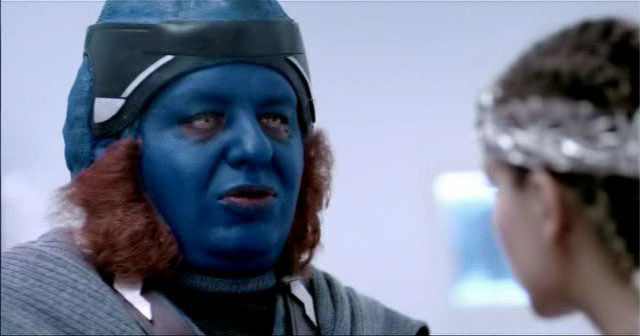
\includegraphics[height=3em]{rendroy2.jpg} \newline
\begin{oneparchoices}
\choice ANOTHERDEGISIM
\choice Amir Tocha
\choice Deneme Method
\choice Rendroy
\end{oneparchoices}
\question Which one is the Arif Isik\newline
\begin{oneparchoices}
\choice 
\includegraphics[height=2em]{faruk.jpg}
\choice 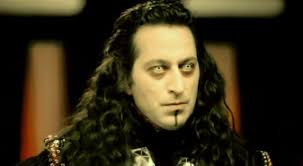
\includegraphics[height=2em]{komutanlogar.jpeg}
\choice 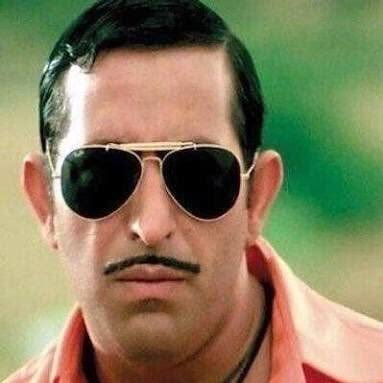
\includegraphics[height=2em]{arifisik.jpg}
\choice 
\includegraphics[height=2em]{216.jpg}
\end{oneparchoices}
\end{questions}
\end{document}